\section{A Matheuristic for the Mothership-Drone Routing Problem with Graphs}\label{Math}
\noindent
This section is devoted to present our matheuristic approach to address the solution of the \MDR. Our motivation comes from the fact that the exact methods presented in the previous section are highly time demanding. Alternatively, the matheuristic provides good quality solution in limited computing times.\\
\noindent
First, we focus on the case in which the mothership can move freely on the continuous space, namely \AMD.
The basic idea of the algorithm is to determine first the sequence of visits to the target graphs in $\mathcal{G}$. This route is obtained replacing each graph in $\mathcal{G}$ by its centroid and then solving a TSP over the neighborhoods of those centroids, namely a XPPN (see \cite{art:Puerto2020}). Then, given such an order of visits, the launching/rendezvous points where the mothership must stop, are determined by solving a \AMD\xspace problem, but limited to one single graph per time, following the sequence previously computed. Successively, the solution so obtained is improved by providing it to the solver as initial partial solution and by solving, once more, another \AMD \ problem, where now we fix the launching/rendezvous points but leave free the variables $w$ that give the sequence of visits to the targets graphs, i.e., without fixing the order of visits.
If the solution so obtained consists in a different order of visit of the graphs with respect to the previous one, the procedure is repeated to generate a new feasible solution. The stopping criterion is to find a solution that does not change with respect to the one obtained in the previous cycle of the algorithm.
In the following, we present the pseudo-code of this algorithm:


\begin{itemize} 
\item[STEP 1] (Centroids of the graphs)\\
- Let $orig$ be the origin/destination of the mothership tour (orange point with label $0$ in Figure \ref{fig:example} [a]).\\
For each graph $g \in \mathcal G$:\\
- identify its centroid $c_g$ and consider its neighborhood defined as the circle $\rho(c_g,2)$ (red points in Figure \ref{fig:example} [a]).
\item[STEP 2] (Order of visit of the graphs)
Determine an order of visit for the graphs in $\mathcal{G}$ by solving the XPPN of the mothership over the set of the neighborhoods associated with the centroids of those graphs (blue tour 0, 1, 2, 3, 4, 0 in Figure  \ref{fig:example} [a]).\\

\item[STEP 3] (launching/rendezvous points location)
Let $\bar{w}_{gg^{'}}, \: \forall g,g^{'} \in \mathcal G$ be the optimal values of the variables $w_{gg^{'}}$ generated by STEP 2.\\
Following this order of visit, set the launching point for the first graph as the depot, then solve the resulting \AMD\xspace limited to the first graph.\\
Repeat the same procedure for the remaining graphs to be visited, by solving \AMD\xspace on one single graph per time, by fixing as launching point of the current graph the rendezvous point of the previous graph.

\item [STEP 4] (Solution update) 
Let $\bar{z}$ be the solution obtained by STEP 3, consisting of the tour of the drone on each target  (Figure \ref{fig:example} [b]), and $\bar{x}_{L}^{g}$, $\bar{x}_{R}^{g} \:\: \forall g \in \mathcal G$ the associated launching/rendezvous points (green and blue points in Figure \ref{fig:example} [b]).\\
Solve the model \AMD\xspace with these launching/rendezvous points but leaving free the $w_{gg^{'}} \:\:\ \forall g,g^{'} \in \mathcal G$ variables and providing to the solver $\bar{z}$ as initial partial solution.
\item [STEP 5]
Let $\hat{z}$ be the updated solution obtained by STEP 4 (again Figure \ref{fig:example} [b] for this illustrative example) and $\hat{w}_{gg^{'}}$ the associated order of visit of the graphs.\\
If the $\hat{w}_{gg^{'}} \neq \bar{w}_{gg^{'}}$ repeat from STEP 3, otherwise stop.
\end{itemize}
\noindent
Note that in the example shown in Figure \ref{fig:example} we solved the \AMD\xspace model by imposing that at least a given percentage of each target must be visited. For this reason the solution consists in drone's missions which visit only part of each graph, as represented by the red segments in Figure \ref{fig:example} [b]. Moreover, for this example, most of the launching/rendezvous points coincide. More precisely, considering Figure \ref{fig:example} [b], the drone starts from the origin and visits part of the first target. The mothership retrieves it at the point labelled 1. From the same point the drone starts the second mission to visit part of the second target and then reaches the mothership at the point labelled 2. From that point the drone starts for visiting the third target meeting the mothership at the point labelled 3. From this latter point the last mission of the drone starts and ends on the mothership at the point labelled 4. Then the mothership with the drone go back to the origin. In this example the solution obtained at STEP 4, by fixing the launching/rendezvous points but not the order of visit, does not change with respect to the one obtained at STEP 3. Thus the procedure stops after the first iteration and provides the solution shown in Figure \ref{fig:example} [b].
The exact resolution of \AMD\xspace can be hard expecially on large instances. For this reason for each call of the solver within the heuristic procedure, we set a maximum number of solutions that the solver can generate before stopping.\\
The procedure adopted for the  \NMD \xspace problem consists in the same steps of the matheuristic presented above for the \AMD \xspace problem but, at STEP 4, the partial solution, given in input to the solver, includes also the values of the variables modelling the routing of the truck on the graph.
%\CV{This procedure is similar for the \NMD  problem by providing, in addition, the variables that model the routing of the truck in the graph as initial partial solution at STEP 4.}


\begin{figure}%
    \centering
    \subfloat[a]{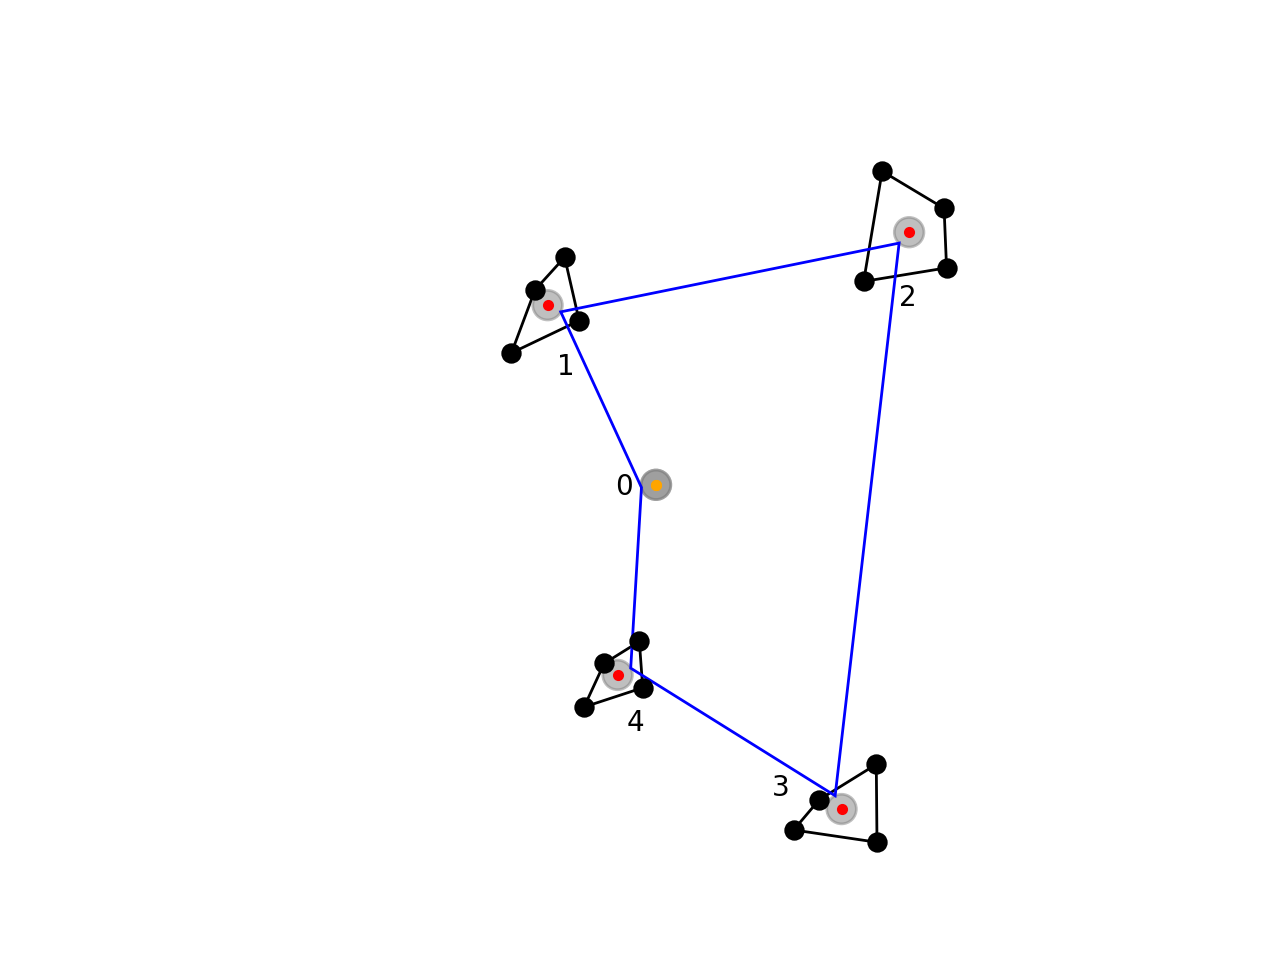
\includegraphics[width=5cm]{./step0.png} }%
    \qquad
    \subfloat[b]{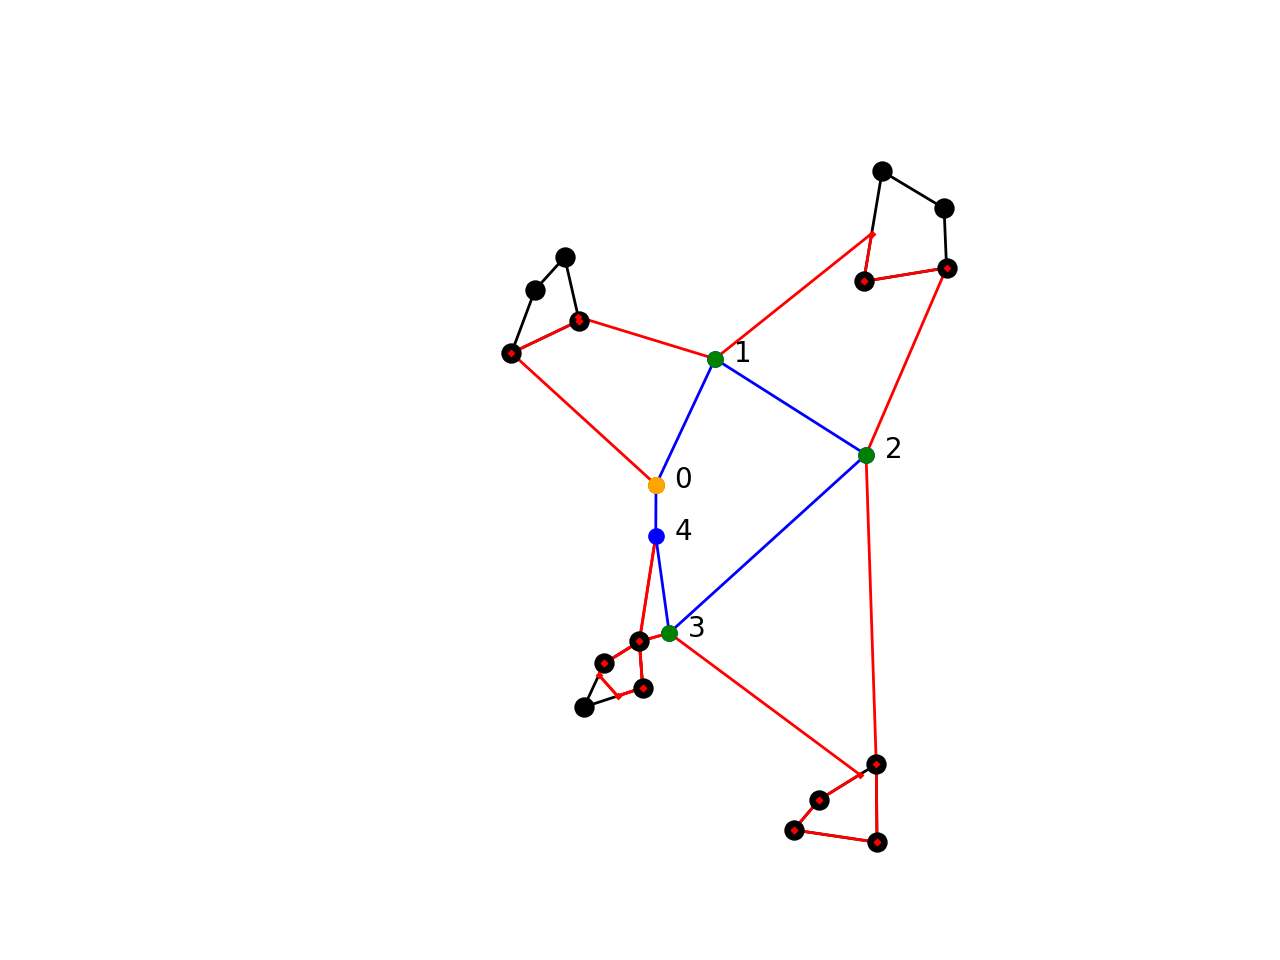
\includegraphics[width=5cm]{./step1.png} }%
    \caption{Illustrative example}%
    \label{fig:example}%
\end{figure}






